\documentclass[dynamic_systems.tex]{subfiles}
\begin{document}

\chapter{Transfer functions}
\tags{}

In \cref{lec:bridge_state_space_to_io}, we briefly introduced the transfer function, a very important dynamic system representation to which we now turn our attention. 
We repeat the definition here.
\tags{}

\input{../_common/tf}

As we learned in \cref{lec:bridge_state_space_to_io}, one can easily convert a state-space model to a (matrix) transfer function model with the formula
\begin{align}
H(s) = C (s I - A)^{-1} B + D.
\end{align}
We also learned that a transfer function and an io ODE are related via the Laplace transform.
The similarities are rather easy to spot, so io ODEs and tranfer functions can be converted to each other via inspection.
\tags{}

\section{Poles and zeros}
\tags{}

Two important types of objects defined from a transfer function $H$ can be used to characterize a system's behavior: \keyword{poles} and \keyword{zeros}.
\tags{}

\begin{Definition}{poles}{}
Let a system have transfer function $H$.
Its \emph{poles} are values of $s$ for which
\begin{align*}
	|H(s)| \rightarrow \infty.
\end{align*}
\end{Definition}

A transfer function written as a ratio has poles wherever the denominator is zero; that is, $s$ for which\footnote{It is common to use this as the definition of a pole, which allows us to talk of ``pole-zero cancellation.'' Occasionally we will use this terminology.}
\maybeeq{
\begin{align*}
	\mathrm{den}\, H(s) = 0.
\end{align*}
}

\begin{Definition}{zeros}{}
Let a system have transfer function $H$.
Its \emph{zeros} are values of $s$ for which
\begin{align*}
	|H(s)| \rightarrow 0.
\end{align*}
\end{Definition}

A transfer function written as a ratio has zeros wherever the numerator is zero; that is, $s$ for which\footnote{It is common to use this as the definition of a zero, which allows us to talk of ``pole-zero cancellation.'' Occasionally we will use this terminology.}
\maybeeq{
\begin{align*}
	\mathrm{num}\, H(s) = 0.
\end{align*}
}

Given a transfer function $H$ with $n$ poles $p_i$ and $\nu$ zeros $z_j$, we can write, for $K\in\mathbb{R}$,
\maybeeq{
\begin{align*}
	H(s) &= K
	\frac{
		\displaystyle\prod_{j=1}^{\nu} s-z_j
	}{%
		\displaystyle\prod_{i=1}^{n} s-p_i
	}.
\end{align*}
}

Poles and zeros can define a single-input, single-output (SISO) system's dynamic model, within a constant.
\tags{}

Recall that, even for multiple-input, multiple-output (MIMO) state-space models, the denominator of every transfer function is the corresponding system's \emph{characteristic equation}---the roots of which dominate the system's response and are equal to its \emph{eigenvalues}.
It is not time to observe a crucial identity.
\tags{}

\begin{Corollary}{poles $=$ eigenvalues $=$ char.\ eq.\ roots}{}
A system's \emph{poles} equal its \emph{eigenvalues} equal its \emph{characteristic equation roots}.
\end{Corollary}

Therefore, everything we know about a system's eigenvalues and characteristic equation roots is true for a system's poles.
This includes that they characterize a system's response (especially its free response) and stability.
\tags{}

\subsection{Pole-zero plots and stability}
\tags{}

The complex-valued poles and zeros dominate system behavior via their values and value-relationships.
Often, we construct a \keyword{pole-zero plot}---a plot in the complex plane of a system's poles and zeros---such as that of \cref{fig:pz_01}.
\tags{}

\begin{figure}
\centering
\begin{tikzpicture}[ 
pole/.pic={\draw[thick] (-3pt,-3pt) -- (3pt,3pt) (3pt,-3pt)--(-3pt,3pt);},
zero/.style={draw,circle,thick,inner sep=3pt},
]
\begin{axis}[
	width=1\linewidth,
	height=.5\linewidth,
  ticks=none,
  axis lines = middle,
  axis line style={->},
  ymin=-10, ymax=10,
  xmin=-10, xmax=10,
	xlabel=$\Re{(s)}$, 
	ylabel=$\Im{(s)}$,
]
  \draw pic at (axis cs:-9,7) {pole};
  \draw pic at (axis cs:-9,-7) {pole};
  \draw pic at (axis cs:0,5) {pole};
  \draw pic at (axis cs:0,-5) {pole};
  \draw pic at (axis cs:-5,0) {pole};
  \draw pic at (axis cs:0,0) {pole};
  \node[zero] at(axis cs:-3,2) {};
  \node[zero] at(axis cs:-3,-2) {};
  \node[zero] at(axis cs:-7,0) {};
  \draw pic at (axis cs:3,6) {pole};
  \draw pic at (axis cs:3,-6) {pole};
  \draw pic at (axis cs:5,0) {pole};
  \node[zero] at(axis cs:7,0) {};
\end{axis}
\end{tikzpicture}
\caption{a pole-zero plot for a system with nine poles and four zeros. In this example, six of the poles are complex-conjugate pairs and three are real. Three are in the right half-plane, making the system unstable. One zero is in the right half-plane, making the system ``minimum phase.''}
\label{fig:pz_01}
\end{figure}



\begin{figure}
\centering
% \pgfplotset{insetsty/.style={
% 	anchor={outer north west},
% 	footnotesize,
% 	width=.2\linewidth,
% 	height=.2\linewidth,
% 	ticks=none,
% 	samples=80,
% 	}}
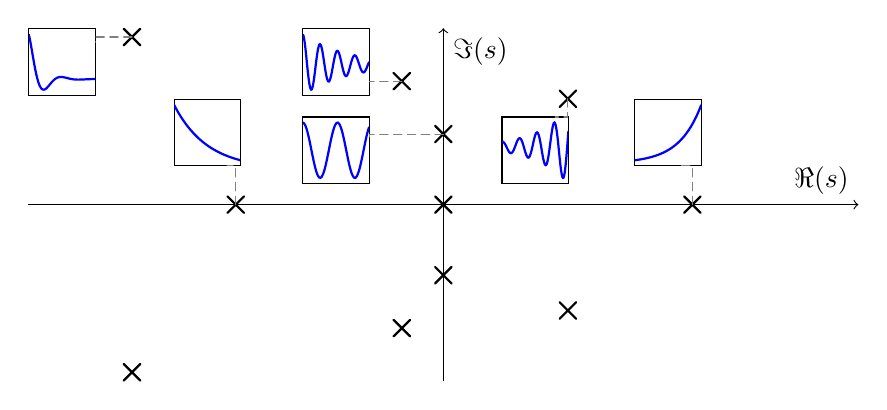
\begin{tikzpicture}[ 
pole/.pic={\draw[thick,line cap=round] (-3pt,-3pt) -- (3pt,3pt) (3pt,-3pt)--(-3pt,3pt);},
zero/.style={draw,circle,thick,inner sep=3pt},
]
\begin{axis}[
	width=1\linewidth,
	height=.5\linewidth,
  ticks=none,
  axis lines = middle,
  axis line style={->},
  ymin=-10, ymax=10,
  xmin=-10, xmax=10,
	xlabel=$\Re(s)$, 
	ylabel=$\Im(s)$,
]
	\coordinate (x1) at (axis cs:-7.5,9.5);
	\coordinate (x2) at (axis cs:-5,0);
	\coordinate (x3) at (axis cs:-1,7);
	\coordinate (x4) at (axis cs:0,4);
	\coordinate (x5) at (axis cs:3,6);
	\coordinate (x6) at (axis cs:6,0);
  \draw pic at (x1) {pole};
  \draw pic at (axis cs:-7.5,-9.5) {pole};
  \draw pic at (x2) {pole};
  \draw pic at (x3) {pole};
  \draw pic at (axis cs:-1,-7) {pole};
  \draw pic at (x4) {pole};
  \draw pic at (axis cs:0,-4) {pole};
  \draw pic at (axis cs:0,0) {pole};
  \draw pic at (x5) {pole};
  \draw pic at (axis cs:3,-6) {pole};
  \draw pic at (x6) {pole};
	\coordinate (insetPosition1) at (rel axis cs:0,1);
	\coordinate (insetPosition2) at (rel axis cs:.175,.8);
	\coordinate (insetPosition3) at (rel axis cs:.33,1);
	\coordinate (insetPosition4) at (rel axis cs:.33,.75);
	\coordinate (insetPosition5) at (rel axis cs:.57,.75);
	\coordinate (insetPosition6) at (rel axis cs:.73,.8);
\end{axis}
\begin{axis}[
	anchor={outer north west},
	width=.2\linewidth,
	height=.2\linewidth,
	ticks=none,
	samples=80,
	smooth,
	at={(insetPosition1)},
	xmin=0,xmax=6,domain=0:6]
	\addplot[mark=none,blue,thick]{(cos(deg(2*x))*exp(-x))};
	\coordinate (inset1Anchor) at (rel axis cs:1,.8);
\end{axis}
\begin{axis}[
	anchor={outer north west},
	width=.2\linewidth,
	height=.2\linewidth,
	ticks=none,
	samples=30,
	smooth,
	at={(insetPosition2)},
	xmin=0,xmax=6,domain=0:6]
	\addplot[mark=none,blue,thick]{exp(-x/3)};
	\coordinate (inset2Anchor) at (rel axis cs:.8,0);
\end{axis}
\begin{axis}[
	anchor={outer north west},
	width=.2\linewidth,
	height=.2\linewidth,
	ticks=none,
	samples=120,
	smooth,
	at={(insetPosition3)},
	xmin=0,xmax=6,domain=0:6]
	\addplot[mark=none,blue,thick]{(cos(deg(4*x))*exp(-x/4))};
	\coordinate (inset3Anchor) at (rel axis cs:1,.2);
\end{axis}
\begin{axis}[
	anchor={outer north west},
	width=.2\linewidth,
	height=.2\linewidth,
	ticks=none,
	samples=50,
	smooth,
	at={(insetPosition4)},
	xmin=0,xmax=6,domain=0:6]
	\addplot[mark=none,blue,thick]{cos(deg(2*x))};
	\coordinate (inset4Anchor) at (rel axis cs:1,.7);
\end{axis}
\begin{axis}[
	anchor={outer north west},
	width=.2\linewidth,
	height=.2\linewidth,
	ticks=none,
	samples=120,
	smooth,
	at={(insetPosition5)},
	xmin=0,xmax=6,domain=0:6]
	\addplot[mark=none,blue,thick]{(cos(deg(4*x))*exp(x/3))};
	\coordinate (inset5Anchor) at (rel axis cs:.8,1);
\end{axis}
\begin{axis}[
	anchor={outer north west},
	width=.2\linewidth,
	height=.2\linewidth,
	ticks=none,
	samples=120,
	smooth,
	at={(insetPosition6)},
	xmin=0,xmax=6,domain=0:6]
	\addplot[mark=none,blue,thick]{exp(x/2)};
	\coordinate (inset6Anchor) at (rel axis cs:.7,0);
\end{axis}
\draw[-,densely dashed,line cap=round,gray] (x1) -| (inset1Anchor);
\draw[-,densely dashed,line cap=round,gray] (x2) |- (inset2Anchor);
\draw[-,densely dashed,line cap=round,gray] (x3) -| (inset3Anchor);
\draw[-,densely dashed,line cap=round,gray] (x4) -| (inset4Anchor);
\draw[-,densely dashed,line cap=round,gray] (x5) |- (inset5Anchor);
\draw[-,densely dashed,line cap=round,gray] (x6) |- (inset6Anchor);
\end{tikzpicture}
\caption{free response contributions from poles at different locations. Complex poles contribute oscillating free responses, whereas real poles do not. Left half-plane poles contribute stable responses that decay. Right half-plane poles contribute unstable responses that grow. Imaginary-axis poles contribute marginal stability.}
\label{fig:pz_02}
\end{figure}

From our identification of poles with eigenvalues and roots of the characteristic equation, we can recognize that each pole contributes an exponential response that oscillates if it is complex.
There are three stability contribution possibilities for each pole $p_i$:
\tags{}
\begin{itemize}
	\item $\Re(p_i) < 0$: a stable, decaying contribution;
	\item $\Re(p_i) = 0$: a marginally stable, neither decaying nor growing contribution; and
	\item $\Re(p_i) > 0$: an unstable, growing contribution.
\end{itemize}
This is explored graphically in \cref{fig:pz_02}.

Of course, we must not forget that a \emph{system's} stability is spoiled with a single unstable pole.
\tags{}

It can be shown that complex poles and zeros always arise as conjugate pairs.
A consequence of this is that the pole-zero plot is always \keyword[real-axis symmetry]{symmetric about the real axis}.
\tags{}

\subsection{Second-order systems}
\tags{}

Second-order response is characterized by a damping ratio $\zeta$ and natural frequency $\omega_n$.
These parameters have clear complex-plane ``geometric'' interpretations, as shown in \cref{fig:pz_03}.
Pole locations are interpreted geometrically in accordance with their relation to rays of constant damping from the origin and circles of constant natural frequency, centered about the origin.
\tags{}

\begin{figure}
\centering
\usetikzlibrary{quotes,angles}
\begin{tikzpicture}[ 
pole/.pic={\draw[thick,line cap=round] (-3pt,-3pt) -- (3pt,3pt) (3pt,-3pt)--(-3pt,3pt);},
zero/.style={draw,circle,thick,inner sep=3pt},
]
\begin{axis}[
	width=1\linewidth,
	% height=.5\linewidth,
  ticks=none,
  axis lines = middle,
  axis line style={->},
  ymin=-.5, ymax=10,
  xmin=-9, xmax=.5,
	xlabel=$\Re(s)$, 
	ylabel=$\Im(s)$,
	axis equal, clip=false,
]
	\addplot[gray,domain=90:180] ({8*cos(\x)}, {8*sin(\x)});
  \draw pic at (axis cs:-9,0) {pole};
  \draw pic at (axis cs:0,9) {pole};
  \draw pic at (axis cs:-6.9282032303,4) {pole};
  \draw pic at (axis cs:-4,6.9282032303) {pole};
  %
  \addplot[->,thick,line cap=round,gray] coordinates
           {(-5.6558542495,5.6578542495) (-5.6568542495,5.6568542495)};
  \node[anchor=north west] at (axis cs:-5.6568542495,5.6568542495) {$\zeta$};
  %
  \draw[gray,dashed] (axis cs:-4,0) -- (axis cs:-4,6.9282032303) -- (axis cs:0,6.9282032303);\draw[gray,dashed] (axis cs:0,0) -- node[midway,anchor=south west,black] {$\omega_n$} (axis cs:-4,6.9282032303);
  \node[anchor=north] at (axis cs:-4,0) {$-\zeta \omega_n$};
  \node[anchor=west] at (axis cs:0,6.9282032303) {$\omega_d$};
  %
  \coordinate (a) at (axis cs:-1,0);
  \coordinate (b) at (axis cs:0,0);
  \coordinate (c) at (axis cs:-4,6.9282032303);
  \draw pic["$\arccos\zeta$",draw=gray,<-,angle eccentricity=1,angle radius=.5cm,anchor=south east] {angle=c--b--a};
  %
  \node[anchor=south west] at (axis cs:-8,0) {$\zeta=1$};
  \node[anchor=west] at (axis cs:0,8) {$\zeta=0$};
  \draw[->,gray,line cap=round] (axis cs:-10.6,0) --node[midway,anchor=south east,black] {$\zeta > 1$} (axis cs:-11,0);
  %
	\coordinate (insetPosition1) at (axis cs:-9.35,.4);
	\coordinate (insetPosition2) at (axis cs:-7.3612159322,4.25);
	\coordinate (insetPosition3) at (axis cs:-4.25,7.3612159322);
	\coordinate (insetPosition4) at (axis cs:-.4,9.35);
\end{axis}
\begin{axis}[
	anchor={outer south},
	width=.28\linewidth,
	height=.28\linewidth,
	ticks=none,
	samples=30,
	smooth,
	at={(insetPosition1)},
	xmin=0,xmax=6,domain=0:6]
	\addplot[mark=none,blue,thick]{exp(-x)};
\end{axis}
\begin{axis}[
	anchor={outer south east},
	width=.28\linewidth,
	height=.28\linewidth,
	ticks=none,
	samples=100,
	smooth,
	at={(insetPosition2)},
	xmin=0,xmax=6,domain=0:6]
	\addplot[mark=none,blue,thick]{(cos(deg(4*x))*exp(-0.7698*x))};
\end{axis}
\begin{axis}[
	anchor={outer south east},
	width=.28\linewidth,
	height=.28\linewidth,
	ticks=none,
	samples=100,
	smooth,
	at={(insetPosition3)},
	xmin=0,xmax=6,domain=0:6]
	\addplot[mark=none,blue,thick]{(cos(deg(4*x))*exp(-.444444*x))};
\end{axis}
\begin{axis}[
	anchor={outer east},
	width=.28\linewidth,
	height=.28\linewidth,
	ticks=none,
	samples=50,
	smooth,
	at={(insetPosition4)},
	xmin=0,xmax=6,domain=0:6]
	\addplot[mark=none,blue,thick]{cos(deg(4*x))};
\end{axis}
\end{tikzpicture}
\caption{second-order free response contributions from poles at different locations, characterized by the damping ratio $\zeta$ and natural frequency $\omega_n$. Constant damping occurs along rays from the origin. Constant natural frequency occurs along arcs of constant radius, centered at the origin.}
\label{fig:pz_03}
\end{figure}

% \begin{problems}

% \subsection{a problem}

% \end{problems}

% \begin{solutions}

% \subsection{a solution}

% \end{solutions}

\end{document}